\documentclass{beamer}
\usepackage{graphicx}
\usepackage{amssymb,amsfonts,amsmath}
% \usepackage{tikz,tkz-euclide}
% \usepackage{subfigure}
% \usepackage{parskip}
% \usetikzlibrary{arrows.meta}
% \usetikzlibrary{calc,patterns}
\usefonttheme[onlymath]{serif}
% biblatex with biber
\usepackage[backend=biber,style=numeric,sorting=none]{biblatex}
\addbibresource{ref.bib}
\usepackage{hyperref}

% 自定义参考文献样式
\DeclareBibliographyDriver{article}{%
  \printnames{author}%
  \setunit{\addspace}%
    \printfield{title}%
    \newunit
  \printfield{journaltitle}%
  \finentry}

% \usetheme{Berlin}
\title{Analysis of Embryo Cell Trajectory with Co-clustering Techniques}
\author{WU Zihan}
\begin{document}
\maketitle
\begin{frame}{Introduction to Embryo Cell Trajectory Analysis}
  \begin{itemize}
    \item Objective: to analyze the trajectory of cells in an embryo and its relationship with cell fate or cell category.
    \item Importance: highlight the importance of understanding cell trajectories for advancing developmental biology and potential medical applications.
  \end{itemize}
\end{frame}

\begin{frame}{Methodology Overview}
  \begin{itemize}
    \item \textbf{Stochastic Modeling:} 
    e.g. Drift-diffusion model, Heston model, etc.
    \item \textbf{Classification and Analysis:} the stochastic models can reveal an expected trajectory pattern and variance characteristics, which can be used to classify embryos and cells based on observable trajectories.
  \end{itemize}
\end{frame}

\begin{frame}{Feature Analysis}
  \begin{itemize}
    \item \textbf{Local Features:} Features that are pointwise and related to time, thus related to fate of the embryo. e.g. curvature, torsion, etc.
    \item \textbf{Global Features:} Features that are related to the overall trajectory of the cell, such as the winding number, basic group, etc.
  \end{itemize}
\end{frame}

\begin{frame}{Co-clustering and Connections}
  % insert matrix.jpeg
  \begin{figure}
    \centering
    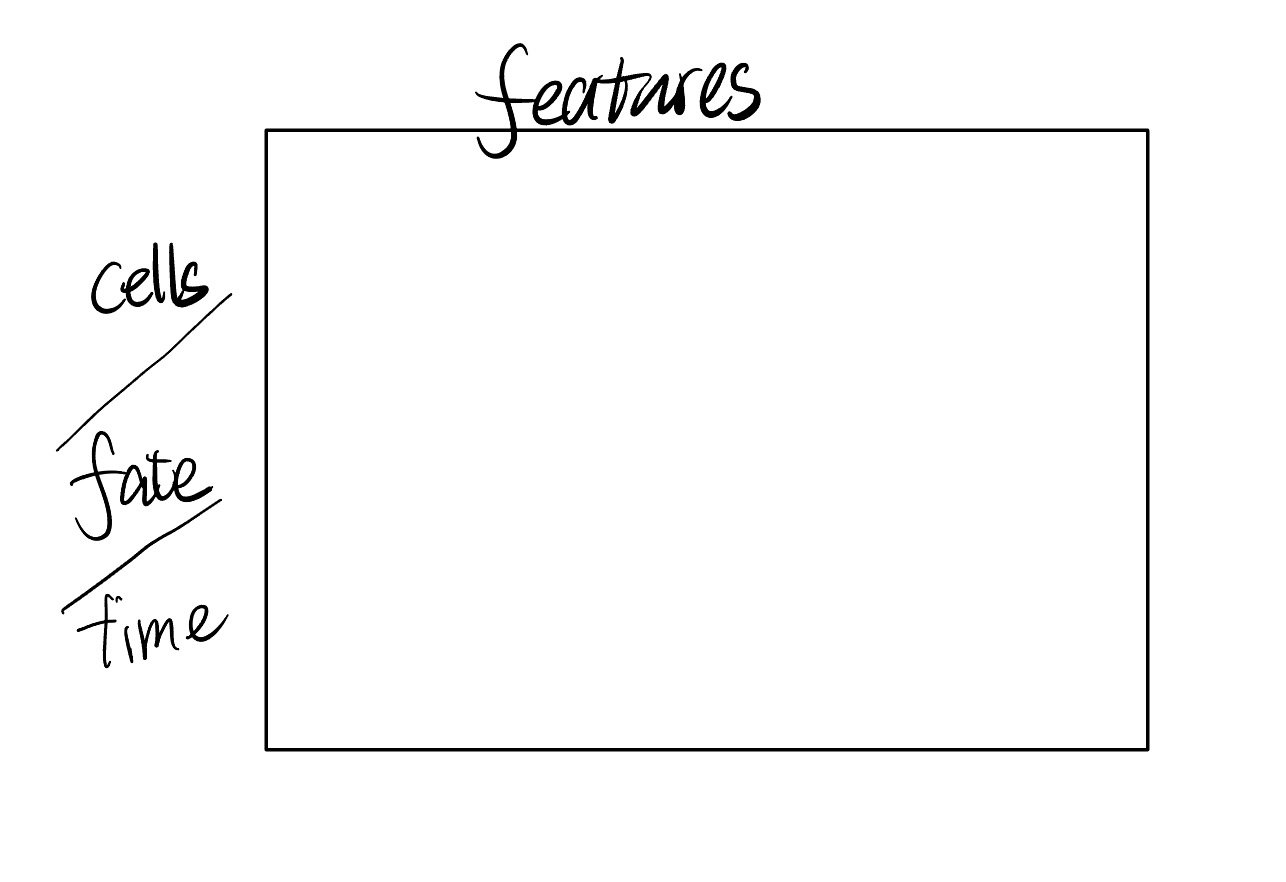
\includegraphics[width=0.5\textwidth]{matrix.jpeg}
    \caption{Co-clustering matrix}
  \end{figure}
\end{frame}

\begin{frame}{Conclusions and Discoveries}
  \begin{itemize}
    \item \textbf{Cell prospective:} e.g. Cell of category A tends to have a trajectory with a higher winding number, etc.
    \item \textbf{Time/Fate prospective:} e.g. During the phase changing, the variance of the trajectory tends be maximum, etc.
  \end{itemize}
\end{frame}

\end{document}